\documentclass{article}
\usepackage{fullpage}
\usepackage{amsmath}
\usepackage{amssymb}
\usepackage{amsthm}
\usepackage{gensymb}
\usepackage{graphicx}
\usepackage[pdftex]{hyperref}
\usepackage{url}
\usepackage{cite}
\usepackage[english]{babel}
\usepackage{algorithm}
\usepackage{algpseudocode}
\usepackage{subcaption}
\usepackage{enumitem}
\usepackage{cleveref}
\crefname{enumi}{goal}{goals}
\usepackage{xargs}                      % Use more than one optional parameter in a new commands
\usepackage[pdftex,dvipsnames]{xcolor}  % Coloured text etc
\usepackage[colorinlistoftodos,prependcaption,textsize=small]{todonotes}
\newcommandx{\unsure}[2][1=]{\todo[inline, linecolor=red,backgroundcolor=red!25,bordercolor=red,#1]{Unsure: #2}}
\newcommandx{\change}[2][1=]{\todo[inline, linecolor=blue,backgroundcolor=blue!25,bordercolor=blue,#1]{To be changed: #2}}
\newcommandx{\info}[2][1=]{\todo[inline, linecolor=OliveGreen,backgroundcolor=OliveGreen!25,bordercolor=OliveGreen,#1]{Info: #2}}
\newcommandx{\idea}[2][1=]{\todo[inline, linecolor=OliveGreen,backgroundcolor=OliveGreen!25,bordercolor=OliveGreen,#1]{Idea: #2}}
\newcommandx{\improvement}[2][1=]{\todo[inline, linecolor=Plum,backgroundcolor=Plum!25,bordercolor=Plum,#1]{To be improved: #2}}
\newcommandx{\thiswillnotshow}[2][1=]{\todo[disable,#1]{#2}}
\usepackage{tikz}
\usepackage{xstring}
\usepackage{pgfplots}
\usepackage{etoolbox}
\usepackage{ifthen}
\usetikzlibrary{arrows,shapes}
\usetikzlibrary{positioning, calc}

\definecolor{hospital}{RGB}{0,0,255}
\definecolor{patient}{RGB}{255,0,0}

\tikzstyle{flow_node}=[circle,draw=black,minimum size=15pt,inner sep=0pt]
\tikzstyle{flow_s}=[fill=green!20]
\tikzstyle{flow_subtask}=[fill=green!80]
\tikzstyle{flow_task}=[fill=red!80]
\tikzstyle{flow_t}=[fill=blue!20]
\tikzstyle{flow_edge}=[->, ultra thick]
\tikzstyle{flow_capacity}=[fill=white, inner sep = 1pt]
\tikzstyle{flow_edge_mincut}=[draw=red]
\tikzstyle{flow_edge_fullcap}=[draw=red]
\tikzstyle{flow_mincut}=[dashed, thick]
\tikzstyle{flow_supply}=[fill=green!80]
\tikzstyle{flow_demand}=[fill=red!80]

\newcommand\ifMaxFlow[4]{
	\begingroup
		\pgfmathsetmacro{\flow}{#1}
		\pgfmathsetmacro{\cap}{#2}
		\pgfmathparse{ifthenelse(\flow == \cap,1,0)}
		\ifdim\pgfmathresult pt= 1 pt
			 #3
			\else
			 #4
		\fi
	\endgroup
}

\newcommand\ifSomeFlow[3]{
	\begingroup
		\pgfmathsetmacro{\flow}{#1}
		\pgfmathparse{ifthenelse(\flow > 0,1,0)}
		\ifdim\pgfmathresult pt= 1 pt
			 #2
			\else
			 #3
		\fi
	\endgroup
}



\graphicspath{{figures/}}

\begin{document}
\title{ADS for Math students in 2018-2019}
\author{Stefan Hugtenburg}
\date{\today}


\maketitle

\section{Introduction}

\begin{frame}
	\frametitle{What is ADS?}
	\pnote{Introduce yourself!}
	
\end{frame}

\begin{frame}
	\frametitle{Solving puzzles using computers!}
	\pause
	\framesubtitle{XKCD Logic Boat: \url{https://xkcd.com/1134}}
	
	\begin{figure}
		\begin{subfigure}{0.45\textwidth}
			\includegraphics[width=\textwidth]{figures/logic_boat_1.png}
		\end{subfigure}
		\hfill
		\pause
		\begin{subfigure}{0.45\textwidth}
			\includegraphics[width=\textwidth]{figures/logic_boat_2.png}
		\end{subfigure}
		\label{fig:XKCD 1134: Logic boat}
	\end{figure}
\end{frame}

\begin{frame}
	\frametitle{Real-world problems}
	\framesubtitle{Queuing in the supermarket}
	\begin{center}
		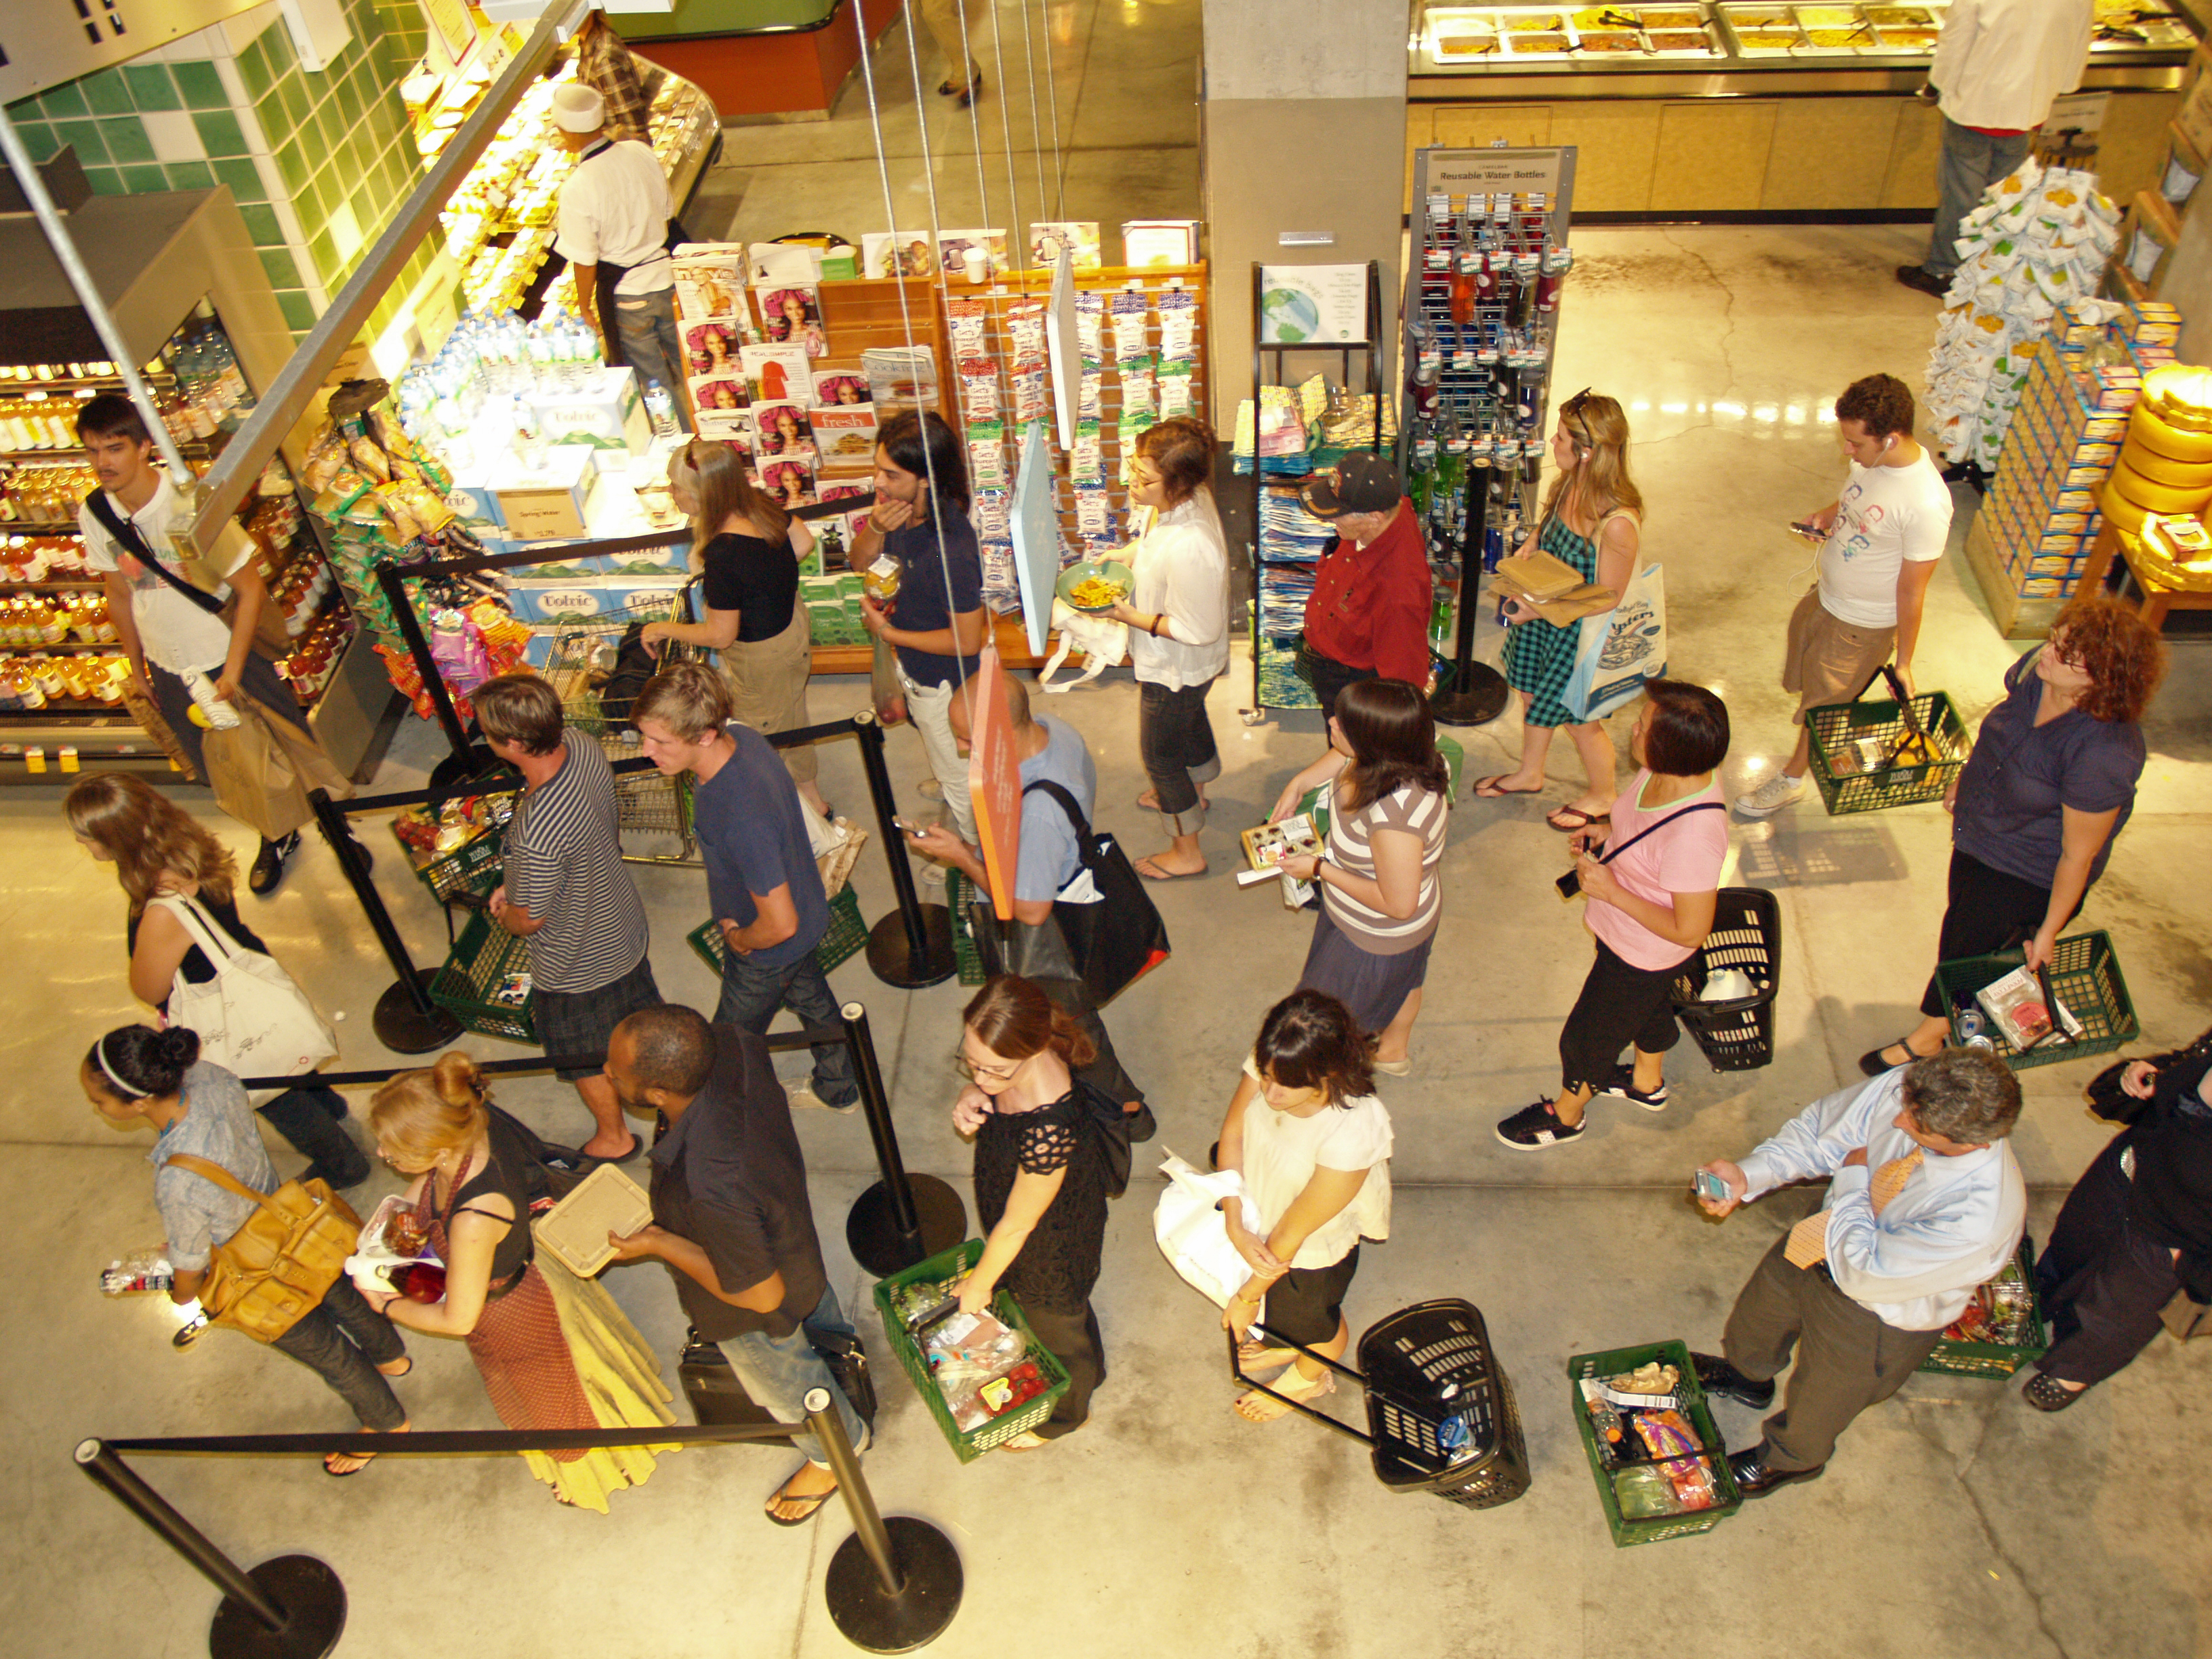
\includegraphics[width=0.6\textwidth]{figures/supermarket.jpg}\\
		\hspace*{15pt}\hbox{\scriptsize Image By:\thinspace{\itshape David Shankbone}}
		%https://commons.wikimedia.org/wiki/File:Waiting_in_line_at_a_food_store.JPG
	\end{center}
	
\end{frame}

\begin{frame}
	\frametitle{Real-world problems}
	\framesubtitle{Finding your way home}
	\begin{center}
		\includegraphics[width=0.6\textwidth]{figures/navigation.jpg}\\
		\hspace*{15pt}\hbox{\scriptsize Image in public domain}
		% https://pxhere.com/en/photo/952741
	\end{center}

\end{frame}

\begin{frame}
	\frametitle{Real-world problems}
	\framesubtitle{Getting the most out of your holiday}
	\begin{center}
		\includegraphics[width=0.5\textwidth]{figures/holidays.jpg}\\
		\hspace*{15pt}\hbox{\scriptsize Images By:\thinspace{\itshape Stefan Hugtenburg}}
	\end{center}
\end{frame}

\begin{frame}
	\frametitle{How do we solve them?}

	\begin{problemblock}{Some real-world problem}
		Given some real-world problem with many bits and pieces of information, how do we solve them?
	\end{problemblock}
	\pause
	\begin{answerblock}{Structure them!}
		\begin{enumerate}
			\item Get the right information out of the problem.
				\pause
				\alert<5->{
			\item Get it into the computer.
			\item Apply an \textit{algorithm} to solve the problem.
			}
				\pause
			\item Get the solution out of the computer.
		\end{enumerate}	
	\end{answerblock}
	\pnote{ADS is (mostly) about step 2 and 3!}
\end{frame}

\subsection{Learning Objectives}
\label{sub:learning_objectives}

\begin{frame}
	\frametitle{So what will I teach you then?}
	\begin{columns}[t]
		\column{0.455\textwidth}
		\begin{block}{Data structures}
			\begin{itemize}
				\item Array-based lists
				\item Linked lists
				\item Queues
				\item Stacks
				\item (Hash)Maps
				\item (Hash)Sets
				\item Trees
				\item Searchtrees
				\item Graphs
			\end{itemize}
		\end{block}	
		\column{0.455\textwidth}
		\pause
		\begin{block}{Algorithms}
			\begin{itemize}
				\item Binary Search
				\item Sorting
				\item Tree traversal
				\item Graph traversal
				\item Shortest paths
			\end{itemize}
		\end{block}	
		\pause
		\begin{alertblock}{All just tools!}
			What I will really teach is you, is how to \textit{solve \st{puzzles} problems}.
		\end{alertblock}	
	\end{columns}
\end{frame}

\begin{frame}
	\frametitle{Rough course-outline}
	\framesubtitle{Know what you are getting into}
	
	\begin{description}[<+->]
		\item[Week 1] Analysing run time and space complexity of algorithms.
		\item[Week 2] Recursive algorithms \& lists
		\item[Week 3] Stacks, Queues \& sorting
		\item[Week 4] Trees \& search trees
		\item[Week 6] Maps \& Graphs
		\item[Week 7] Graph algorithms
		\item[Week 8] P vs NP \& exam prep
	\end{description}
\end{frame}

\begin{frame}
	\frametitle{Short survey time!}
	Just for my curiosity.
	\begin{itemize}
		\item What are you excited about?
		\item Why choose this course?
		\item Programming experience?
	\end{itemize}
	% TODO: [stefan] Find out what survey tool to use. (Fri 04 Jan 2019 04:39:19 PM CET)
\end{frame}

\section{Learning Objectives}
\label{sec:learning_objectives}

The main learning objectives of the course are formulated as follows.

After this course, the student is able to:
\begin{enumerate}[label=\textbf{LO-\arabic*}]
	\item define big-Oh, Omega and Theta notation for complexity of code. \label{lo:notation}
	\item analyse the run time complexity of (recursive) (pseudo)code. \label{lo:runtime}
	\item analyse the space complexity of (recursive) (pseudo)code. \label{lo:space}
	\item define hash and equality functions for custom classes in python. \label{lo:hash}
	\item analyse and implement (doubly) linked lists, arraylists, stacks, and queues. \label{lo:list} \label{lo:queue}
		\label{lo:stack}
	\item describe and implement a variety of sorting algorithms (bubble sort, selection sort, merge sort, 
		quicksort). \label{lo:sort}
	\item analyse and implement search trees, such as binary search trees, AVL trees, and red-black trees. \label{lo:tree}
	\item analyse and implement priorityqueues and heaps. \label{lo:pqueue} \label{lo:heap}
	\item analyse and implement hash sets and maps. \label{lo:set} \label{lo:map}
	\item prove claims about trees and graphs and algorithms operating on them. \label{lo:prove}
	\item analyse and implement graph algorithms, such as: Breadth-First Search (BFS), Depth-First Search (DFS), Dijkstra, and
		Prim.\label{lo:graph}
	\item select the right datastructure for a given problem with certain run time and memory requirements. \label{lo:selecting}
\end{enumerate}

For every lecture we describe which of these we address and how we break this down in smaller learning objectives
specific to that lecture.


\section{Course layout}
\label{sec:course_layout}

In this section we describe the new course layout, focusing on what learning objectives are covered in the different
lectures, homeworks, and exams.

Table~\ref{tab:schedule} provides an overview of the lecturing schedule for the course, each lecture is discussed in
more detail below, where we also describe what the tutorial and assignments are for the corresponding week. For every
lecture and tutorial there is a lesson plan, including learning objectives, the intermezzo topic (in case of lectures),
and how much time is spent on different topics. For every weekly assignment there is also an indicated amount of time
students are expected to spend on them.

\begin{table}[htpb]
	\centering
	\caption{The course schedule, vertical lines indicate which material is tested in the exam in the week after that
	lecture. E.g. The line after lecture 8 indicates all material up to lecture 8 can be tested in the exam in week 5.}
	\label{tab:schedule}
	\begin{tabular}{c | r | l}
		Week & Lecture & Topic \\
		\hline
		1 & Lecture 1 & Course overview \& introduction to complexity\\
		1 & Lecture 2 & Complexity notation \& Space complexity  \\
		2 & Lecture 3 & Recursion \& the Master Method\\
		2 & Lecture 4 & Equality and lists \\
		3 & Lecture 5 & Stacks and Queues\\
		3 & Lecture 6 & Sorting \\
		4 & Lecture 7 & Trees and heaps \\
		4 & Lecture 8 & Heaps and searchtrees \\
		\hline
		6 & Lecture 9 & Hashmaps and hashsets\\
		6 & Lecture 10 & Introduction to graphs \& graph traversal\\
		7 & Lecture 11 & Dijkstra \& A* \\
		7 & Lecture 12 & MSTs \\
		8 & Lecture 13 & P vs NP\\
		8 & Lecture 14 & Exam prep\\
		\hline
	\end{tabular}
\end{table}

\newpage
\subsection{Week 1}
\label{sub:week_1}

\subsubsection{Lecture 1: Counting operations \& big-Oh analysis}
\label{sub:lecture_1}

This lecture introduces the course material and presents a course overview. 

\hfill\\
\textbf{Learning Objectives:}\\
We start with \cref{lo:runtime}
of the course, more specifically after this lecture the student is able to:
\begin{itemize}
	\item count primitive operations in iterative pieces of code.
	\item derive a total expression in terms of primitives for a piece of code.
	\item describe the notion of big-Oh in complexity theory.
	\item prove a function is of a certain big-Oh complexity.
	\item order a set of functions based on their complexity.
\end{itemize}

\hfill\\
\textbf{Intermezzo:}\\
\improvement{Look this up concretely, I remember something about some significant increase in speed in some ruby method
that the standard library uses a lot}

\hfill\\
\textbf{Lecture plan:}\\
\begin{description}
	\item[5 min] Introduction and what do students expect from the course?
	\item[5 min] Why is ADS cool/important?
	\item[3 min] What will I teach them? (L.O.s in plain language)
	\item[5 min] Short survey to audience: what do they want to learn, what not? Why choose this subject?
	\item[12 min] Course set-up: exams, labs (TAs), tutorials, lectures, weblab, e-mail address, weekly assignments, the
		book.
	\item[15 min] Python recap (interactive), maps, sets, lists, classes.
	\item Break time
	\item[5 min] Intermezzo
	\item[5 min] Counting primitives in for-loop and nested for-loop.
	\item[5 min] Counting in nested with i= 0 to n, j = i to n.
	\item[5 min] Comparing runtimes experimentally (constant, linear, quadratic, exponential, factorial).
	\item[3 min] Formal notation for big-Oh.
	\item[7 min] A big-Oh proof for one of the examples studied earlier.
	\item[1 min] The notion of polynomial run time.
	\item[5 min] Revisit the previous code examples.
	\item[5 min] The notion of tightest bound and comparing functions.
	\item[4 min] Short survey about the lecture: what was unclear, what was good, what could be better?
\end{description}

\subsubsection{Lecture 2: Complexity notation, space complexity \& an introduction to recursion}
\label{sub:lecture_2}

\hfill\\
\textbf{Learning Objectives:}\\
This lecture concerns \cref{lo:notation,lo:runtime,lo:space} of the course, more specifically after this lecture the
student is able to:
\begin{itemize}
	\item describe the notion of $\Theta$, $\Omega$ in complexity theory.
	\item derive the right big-Oh notation for an iterative piece of code.
	\item describe the time and space complexity of some common python functions.
	\item derive the space complexity of algorithms.
	\item derive a recurrence relation for time and space from a recursive piece of code.
	\item prove the run time complexity of a recursive piece of code using repeated unfolding and induction.
\end{itemize}

\hfill\\
\textbf{Intermezzo:}\\
The big-Oh race of matrix multiplication.

\hfill\\
\textbf{Lecture problem:}\\
Searching in a sorted list. (Only second half of the lecture)

\hfill\\
\textbf{Lecture plan:}\\
\begin{description}
	\item[5 min] Notes on the admin related side \& questions from students.
	\item[5 min] Recap of last lecture, reminder of big-Oh and one example of it.
	\item[10 min] Python standards like \texttt{in} for a list, \texttt{range}, and list comprehension.
		\unsure{Maybe other functions/standards are more suitable?}
	\item[5 min] big-$\Theta$ and big-$\Omega$: why care about those?
	\item[3 min] Introduction to space complexity.
	\item[5 min] What happens with memory under the hood of python? Heap vs stack (short and not too technical)
	\item[7 min] Code examples, including: why we ignore the input.
	\item[5 min] Relations between time and space.
	\item Break time
	\item[5 min] Intermezzo
	\item[2 min] Introduction to today's problem.
	\item[3 min] Introduction to recursion.
	\item[8 min] Binary search: how does it work, what is the rec. equation for run time and space?
	\item[7 min] What is such a recurrence equation? Generalise to recursion trees (fibonacci?)
	\item[15 min] Solving a rec. equation. First repeatedly unfold, then prove by induction. Do this for BS.
	\item[5 min] Short survey about the lecture: what was unclear, what was good, what could be better?
\end{description}

\subsubsection{Tutorial 1: Complexity notation, space complexity}
\label{ssub:tutorial_1_complexity_notation_space_complexity}

\hfill\\
\textbf{Plan:}\\
\begin{description}
	\item[10 min] Exercise C1.18 from the book.
	\item[10 min] Exercise C1.15 from the book.
	\item[10 min] Iterative minmax function that returns both.
	\item[15 min] Recursive minmax function that returns both.
	\item Break time
	\item[10 min] Prove something is $\Theta(n^2)$.
	\item[5 min] Prove that $\log n$ is $O(n^c)$ for any $c > 0$.\unsure{Not sure if I want this, might not be needed for
		math students.}
	\item[5 min] Analyse iterative minmax.
	\item[10 min] Analyse recursive minmax.
	\item[10 min] Space complexity of iterative and recursive minmax.
	\item[5 min] Short survey about the tutorial: what was unclear, what was good, what could be better?
\end{description}

\newpage
\subsubsection{Assignment 1: Deadline Sunday before week 2}
\label{ssub:assignment_1}
\unsure{Should be about 7 hours of work. Currently planned: 6 hours. For the first week this may be okay.}

\hfill\\
\textbf{Analysis:}\\
\begin{description}
	\item[10 min] Order sets of functions by big-Oh, determine if functions are $\Theta(f(n))$ or not.
	\item[] Give T(n) and determine big-Oh. \unsure{Look into ways to auto-grade without making it MC.}
		\begin{description}
			\item[5 min] Search in $O(n)$ list.
			\item[5 min] Cartesian product in $O(n^2)$ sets.
			\item[5 min] Matrix multiplication in $O(n^3)$.
			\item[10 min] Recursive fibonacci (impossible to do properly at the level of this course, but we can do it by
				hinting that T(n-2) is O(T(n-1))).
			\item[10 min] Recursive product.
			\item[15 min] Code fragment 4.10 from the book. Answer is $O(n)$ is already given.
		\end{description}
	\item[30 min] 4 rec. equations for which closed form and big-Oh should be determined.
	\item[15 min] 5 MC (exam-level) questions.
	\item[15 min] Big-Oh proof.
\end{description}

\hfill\\
\textbf{Implementation:}\\
\begin{description}
	\item[45 min] Basic OOP-skills in python. \idea{Points and triangles?}
	\item[15 min] IndexOf method for lists.
	\item[20 min] Dict$<$Key, Set$>$ find all keys for which a certain $v$ is in the set of values.
	\item[20 min] Something with exception handling/throwing.
	\item[20 min] Something that requires a tuple of return values.
	\item[20 min] Binary search.
	\item[40 min] Towers of Hanoi (C4.14).
	\item[30 min] Exercise C4.18.
	\item[30 min] Exercise C4.19.
\end{description}

\hfill\\
\textbf{Extra challenges:}\\
\begin{description}
	\item[40 min] FPC: number of zeroes in factorial \unsure{Maybe?}
\end{description}

\newpage
\subsection{Week 2}
\label{sub:week_2}

\subsubsection{Lecture 3: Recursion \& the Master Method}
\label{sub:lecture_3}

\hfill\\
\textbf{Learning Objectives:}\\
This lecture concerns \cref{lo:runtime,lo:space} of the course, more specifically after this lecture the student is able
to:
\begin{itemize}
	\item describe the solution to solving the closest pair of points problem.
	\item derive a recurrence relation for time from a recursive piece of code.
	\item prove the run time complexity of a recursive piece of code using the master method.
\end{itemize}

\hfill\\
\textbf{Intermezzo:}\\
\improvement{Maybe something map reduce?}

\hfill\\
\textbf{Lecture problem:}\\
Closest pair of points.

\hfill\\
\textbf{Lecture plan:}\\
\begin{itemize}
	\item[5 min] Notes on the admin related side \& questions from students.
	\item[5 min] Recap of last lecture, reminder of recurrence equations etc.
	\item[35 min] Closest-pair of points problem and solution.
	\item Break time
	\item[5 min] Intermezzo
	\item[10 min] The master method: how does it work?
	\item[15 min] Examples of applying the master method.
	\item[10 min] Back to closest-pair of points.
	\item[5 min] Short survey about the lecture: what was unclear, what was good, what could be better?
\end{itemize}

\newpage
\subsubsection{Lecture 4: Equality, and lists}
\label{sub:lecture_4}

\hfill\\
\textbf{Learning Objectives:}\\

This lecture concerns \cref{lo:hash,lo:list} of the course, more specifically after this lecture the student is able
to:
\begin{itemize}
	\item describe the differences between linked lists and position-based lists.
	\item describe the implementation of linked lists and arraylists.
	\item select the right type of list given a use case.
	\item explain the need for equality function for a custom class.
\end{itemize}

\hfill\\
\textbf{Intermezzo:}\\
\unsure{Something vaguely related to lists?}

\hfill\\
\textbf{Lecture problem:}\\
A queue (linked list) like in the supermarket and maybe goods in the supermarket that are like an array? \unsure{needs
work}

\hfill\\
\textbf{Lecture plan:}\\
\begin{itemize}
	\item[5 min] Notes on the admin related side \& questions from students.
	\item[5 min] Recap of last lecture, master method for recursion.
	\item[5 min] Introduction to today's topic: lists and different use cases.
	\item[15 min] Analysing the python list implementation: array-based. Adding, removing, searching.
	\item[10 min] Amortised run time when growing an array list.
	\item[5 min] Introduction to alternative implemention: linked-list.
	\item Break time
	\item[5 min] Intermezzo
	\item[15 min] An alternative implementation: singly and doubly linked-list. Adding, removing, searching.
	\item[5 min] Space and time considerations for different types of lists.
	\item[5 min] Back to our problem of today and solving it.
	\item[10 min] Putting custom objects into such lists, the need for equality functions.
	\item[5 min] Short survey about the lecture: what was unclear, what was good, what could be better?
\end{itemize}

\newpage
\subsubsection{Tutorial 2: Recursion \& lists}
\label{ssub:tutorial_1_complexity_notation_space_complexity}

\hfill\\
\textbf{Plan:}\\
\begin{itemize}
	\item[15 min] Exercise P4.24 from the book.
	\item[10 min] Exercise C1.15 from the book.
	\item[10 min] Exercise R7.1 from the book.
	\item[10 min] Exercise C7.28 from the book.
	\item Break time
	\item[10 min] Implementing equals functions.
	\item[15 min] Practice with the master method (3 exercises).
	\item[10 min] Analyse algorithm that uses linked-lists.
	\item[5 min] Given a use case, decide between LL and Array-based.
	\item[5 min] Short survey about the tutorial: what was unclear, what was good, what could be better?
\end{itemize}


\newpage
\subsubsection{Assignment 2: Deadline Sunday before week 3}
\label{ssub:assignment_2}

\hfill\\
\textbf{Analysis:}\\
\begin{description}
	\item[45 min] 5 rec. equations to solve using the master method.
	\item[15 min] 2 rec. equations to solve using repeated unfolding.
	\item[10 min] 1 rec. equations to solve using repeated unfolding + induction.
	\item[] Give T(n) and determine big-Oh. \unsure{Look into ways to auto-grade without making it MC.}
		\begin{description}
			\item[10 min] 2 simple recursions.
			\item[10 min] More complicated recursion.
			\item[15 min] Something with array-based lists.
			\item[15 min] Same thing, but with with linked-lists.
		\end{description}
	\item[15 min] 5 MC (exam-level) questions.
	\item[15 min] Big-Omega proof.
\end{description}

\hfill\\
\textbf{Implementation:}\\
\begin{description}
	\item[60 min] Closest-pair of points.
	\item[45 min] Given implementation of singly-linked list, make it doubly-linked.
	\item[90 min] Circularly-linked list (not covered in lecture, so needs to be built up well!)
	\item[30 min] \hfill\\\unsure{Some problem that needs solving using only a list (maybe something with a simple unsorted queue) that
		favours a linked-list over an array-based one.}
	\item[45 min] \hfill\\\unsure{Maybe something like the stuff explained in 7.6?}
\end{description}

\newpage
\subsection{Week 3}
\label{sub:week_3}

\subsubsection{Lecture 5: Stacks and queues}
\label{sub:lecture_5}

\hfill\\
\textbf{Learning Objectives:}\\
This lecture concerns \cref{lo:stack,lo:queue} of the course, more specifically after this lecture the student is able
to:
\begin{itemize}
	\item define the interface of a stack and of a queue.
	\item describe the differences between a stack and a queue.
	\item implement one interface in terms of the other (i.e. a stack from 2 queues or a queue from 2 stacks).
	\item select the right one (either a stack or a queue) given a use case.
\end{itemize}

\hfill\\
\textbf{Intermezzo:}\\
Routers: fifo in routing.

\hfill\\
\textbf{Lecture problem:}\\
Parsing LaTeX (stacks) and the supermarket registry (queues).

\hfill\\
\textbf{Lecture plan:}\\
\begin{itemize}
	\item[5 min] Notes on the admin related side \& questions from students.
	\item[5 min] Recap of last lecture, reminder of different types of lists.
	\item[5 min] Introduce problem of parsing TeX.
	\item[5 min] Stack properties.
	\item[5 min] Stack implementation: linked-list based.
	\item[10 min] Using a stack to parse our TeX.
	\item[5 min] Introduce problem of supermarket queuing (and maybe traffic jams).
	\item[5 min] Queue properties.
	\item Break time
	\item[5 min] Intermezzo
	\item[5 min] Queue implementation: linked-list based.
	\item[5 min] Solving the problem of the supermarket.
	\item[10 min] Queue implementation: circularly-linked list.
	\item[5 min] Whoops, we made a Deque now.
	\item[10 min] Using a Stack as a Queue.
	\item[5 min] Short survey about the lecture: what was unclear, what was good, what could be better?
\end{itemize}

\newpage
\subsubsection{Lecture 6: Sorting}
\label{sub:lecture_6}

\hfill\\
\textbf{Learning Objectives:}\\

This lecture concerns \cref{lo:sort} of the course, more specifically after this lecture the student is able
to:
\begin{itemize}
	\item compare and implement bubble sort, selection sort, merge sort, bucket sort, and quicksort.
	\item combine different sorting strategies.
	\item select the right type of sorting given a use case.
\end{itemize}

\hfill\\
\textbf{Intermezzo:}\\
Algorithms to Live by.

\hfill\\
\textbf{Lecture problem:}\\
Remember Binary Search? Only good if the list is sorted. \improvement{Needs a nice story}

\hfill\\
\textbf{Lecture plan:}\\
\begin{itemize}
	\item[5 min] Notes on the admin related side \& questions from students.
	\item[5 min] Recap of binary search.
	\item[5 min] Introduction to today's topic: sorting.
	\item[10 min] Bubble-sort: idea, algorithm, and analysis.
	\item[15 min] Selection-sort: idea, algorithm, and analysis.
	\item[5 min] Bucket-sort: idea, algorithm, and analysis.
	\item Break time
	\item[5 min] Intermezzo
	\item[15 min] Merge-sort: idea, algorithm, and analysis (master method).
	\item[15 min] Quick-sort: idea, algorithm, and analysis.
	\item[5 min] Recap: what did we see, how are they different?
	\item[5 min] Short survey about the lecture: what was unclear, what was good, what could be better?
\end{itemize}

\newpage
\subsubsection{Tutorial 3: Stacks, Queues, Sorting}
\label{ssub:tutorial_3}

\hfill\\
\textbf{Plan:}\\
\begin{itemize}
	\item[15 min] Exercise C6.20 from the book.
	\item[10 min] Exercise C6.26 from the book.
	\item[15 min] Implement Selection-sort.
	\item[5 min] Sorting with a key-function in python.
	\item Break time
	\item[5 min] Questions about popping/pushing from/to stacks/queues.
	\item[5 min] Analyse C6.26.
	\item[10 min] Exercise R12.10.
	\item[5 min] Exercise R12.15.
	\item[15 min] Analysing random quick-sort? \unsure{I might also be interested in teaching something like 12.4.1}
	\item[5 min] Short survey about the tutorial: what was unclear, what was good, what could be better?
\end{itemize}


\newpage
\subsubsection{Assignment 3: Deadline Sunday before week 4}
\label{ssub:assignment_3}

\hfill\\
\textbf{Analysis:}\\
\begin{description}
	\item[] Give T(n) and determine big-Oh. \unsure{Look into ways to auto-grade without making it MC.}
		\begin{description}
			\item[10 min] 2 simple recursions.
			\item[10 min] More complicated recursion.
			\item[15 min] Something with stacks.
			\item[15 min] Something with deques.
			\item[10 min] Sorting algorithm A.
			\item[10 min] Sorting algorithm B.
			\item[10 min] Sorting algorithm C.
		\end{description}
	\item[15 min] 5 MC (exam-level) questions.
	\item[10 min] 2 rec. equations to solve using the master method.
	\item[10 min] 1 rec. equations to solve using repeated unfolding + induction.
	\item[10 min] Big-Theta proof.
\end{description}

\hfill\\
\textbf{Implementation:}\\
\begin{description}
	\item[30 min] Implement a Stack with Queues (explained in lecture).
	\item[45 min] Implement a Queue with Stacks (not explained in lecture).
	\item[45 min] Implement merge-sort.
	\item[45 min] Implement quick-sort.
	\item[30 min] \hfill\\\unsure{Some problem that needs solving using only queues and stacks, students should select
		which.}
	\item[45 min] \hfill\\\unsure{A sorting algorithm not explained in the lecture.}
	\item[30 min] Implement sorting on a linked-list structure of some kind (partially recap).
\end{description}

\newpage
\subsection{Week 4}
\label{sub:week_4}

\subsubsection{Lecture 7: Trees}
\label{sub:lecture_7}

\hfill\\
\textbf{Learning Objectives:}\\

This lecture concerns \cref{lo:tree} of the course, more specifically after this lecture the student is able
to:
\begin{itemize}
	\item describe the interface of a tree.
	\item construct basic tree-traversal algorithms (like post-order).
	\item analyse the run time complexity of basic tree-traversal algorithms.
\end{itemize}

\hfill\\
\textbf{Intermezzo:}\\
\unsure{Something fun with trees}

\hfill\\
\textbf{Lecture problem:}\\
Parsing mathematical expressions.

\hfill\\
\textbf{Lecture plan:}\\
\begin{itemize}
	\item[5 min] Notes on the admin related side \& questions from students.
	\item[5 min] Recap of last lecture, reminder of different types sorting.
	\item[5 min] Introduce problem of parsing math, relate back to recursion trees.
	\item[5 min] Tree properties: parents, children, ancestors, descendants, root.
	\item[5 min] Tree implementation: linked structure.
	\item[10 min] Tree ADT: methods like: size, leafs, height.
	\item[10 min] A binary tree.
	\item Break time
	\item[5 min] Intermezzo
	\item[10 min] Alternative implementation: array-based.
	\item[10 min] Tree-traversals (one implemented, the others described only).
	\item[5 min] Solving the parsing problem (what traversal order do we need?)
	\item[10 min] Introduction to heap-structure: binary tree with special properties.
	\item[5 min] Short survey about the lecture: what was unclear, what was good, what could be better?
\end{itemize}

\newpage
\subsubsection{Lecture 8: Heaps \& Searchtrees}
\label{sub:lecture_8}

\hfill\\
\textbf{Learning Objectives:}\\

This lecture concerns \cref{lo:tree,lo:heap} of the course, more specifically after this lecture the student is able
to:
\begin{itemize}
	\item describe the properties of a balanced tree.
	\item construct a binary search tree by repeatedly applying the insert operation.
	\item analyse the run time complexity of binary search tree algorithms.
\end{itemize}

\hfill\\
\textbf{Intermezzo:}\\
Databases and their use of B-trees.

\hfill\\
\textbf{Lecture problem:}\\
\improvement{Fun story that requires a priority queue.}

\hfill\\
\textbf{Lecture plan:}\\
\begin{itemize}
	\item[5 min] Notes on the admin related side \& questions from students.
	\item[5 min] Recap of trees and heaps.
	\item[5 min] Introduce the PQ problem.
	\item[15 min] Up and down bubbling.
	\item[10 min] Analysing the priorityqueue we just created.
	\item[5 min] Solve our PQ problem.
	\item Break time
	\item[5 min] Intermezzo
	\item[5 min] Problem with sorted tree.
	\item[15 min] Introduce notion of binary search tree: insertions/deletions.
	\item[15 min] Extend to Multiway search tree.
	\item[5 min] Short survey about the lecture: what was unclear, what was good, what could be better?
\end{itemize}

\newpage
\subsubsection{Tutorial 4: Trees}
\label{ssub:tutorial_4}

\hfill\\
\textbf{Plan:}\\
\begin{itemize}
	\item[10 min] Implement something like: countLeaves() for a tree.
	\item[10 min] Implement something like: depth() for a tree.
	\item[15 min] Implement searching for an item in a binary search tree.
	\item[10 min] Implement searching for an item in a multiway search tree.
	\item Break time
	\item[5 min] Exercise R8.16.
	\item[10 min] Exercise R8.34.
	\item[10 min] Exercise C8.43.
	\item[5 min] Questions about insertion/deletion from heaps.
	\item[5 min] Exercise R11.16.
	\item[5 min] Exercise R11.21a.
	\item[5 min] Short survey about the tutorial: what was unclear, what was good, what could be better?
\end{itemize}


\newpage
\subsubsection{Assignment 4: Deadline Sunday before week 5}
\label{ssub:assignment_4}

\hfill\\
\textbf{Analysis:}\\
\begin{description}
	\item[] Give T(n) and determine big-Oh. \unsure{Look into ways to auto-grade without making it MC.}
		\begin{description}
			\item[5 min] 1 simple recursions.
			\item[10 min] More complicated recursion.
			\item[10 min] Sorting algorithm D.
			\item[45 min] Tree algorithms!
		\end{description}
	\item[15 min] 5 MC (exam-level) questions.
	\item[10 min] 2 use cases with the question: what data structure would you use and why?
	\item[10 min] 2 rec. equations to solve using the master method.
	\item[10 min] 1 rec. equations to solve using repeated unfolding + induction.
	\item[10 min] Big-Omega proof.
\end{description}

\hfill\\
\textbf{Implementation:}\\
\begin{description}
	\item[45 min] Tree traversals.
	\item[45 min] Implement some heap bubbling.
	\item[90 min] Implement a (2,4)-tree.
	\item[30 min] Extend it to a (3,5)-tree.
	\item[30 min] \hfill\\\unsure{Some problem that needs solving using a PQ, maybe a nice greedy problem? We can give
		most of the idea away, students should just implement it.}
	\item[30 min] Implement selection-sort.
	\item[30 min] Implement radix-sort.
\end{description}

\newpage
\subsection{Week 6}
\label{sub:week_6}

\subsubsection{Lecture 9: Hashsets and maps}
\label{sub:lecture_9}

\hfill\\
\textbf{Learning Objectives:}\\
This lecture concerns \cref{lo:map,lo:set} of the course, more specifically after this lecture the student is able
to:
\begin{itemize}
	\item list the requirements a hash functions should fulfill.
	\item implement an equality and hash function for a custom python class.
	\item describe the operations of the \texttt{dict} datastructure in python.
	\item describe the interface of a map.
	\item describe the differences between a hashset and a hashmap.
	\item describe how hash conflicts are handled by these datastructures.
\end{itemize}

\hfill\\
\textbf{Intermezzo:}\\
The importance of good hash funtions, link to assignment

\hfill\\
\textbf{Lecture problem:}\\
Zesje: matching students to submissions.

\hfill\\
\textbf{Lecture plan:}\\
\begin{itemize}
	\item[5 min] Notes on the admin related side \& questions from students.
	\item[5 min] Recap of last lecture, sorted trees.
	\item[5 min] Introduce problem of matching objects to objects. We all know about dictionaries already, but...
	\item[5 min] Properties of hash functions (one or two examples)
	\item[5 min] Implementing a hash function in python.
	\item[20 min] What does a dict do in python: hash conflicts, internal data structures etc.
	\item Break time
	\item[10 min] Intermezzo
	\item[5 min] Sets in python: maps without keys.
	\item[5 min] Solving the problem of zesje.
	\item[20 min] Sorted maps and multimaps
	\item[5 min] Short survey about the lecture: what was unclear, what was good, what could be better?
\end{itemize}

\newpage
\subsubsection{Lecture 10: Introduction to graphs}
\label{sub:lecture_8}

\hfill\\
\textbf{Learning Objectives:}\\
\begin{itemize}
	\item define basic graph components (vertices, edges, directedness).
	\item prove certain properties about graphs.
	\item describe the operation of DFS and BFS.
	\item select the right traversal algorithm for a given use case.
	\item describe how DFS and BFS can be used to detect cycles in a graph.
\end{itemize}

\hfill\\
\textbf{Intermezzo:}\\
Graph databases

\hfill\\
\textbf{Lecture problem:}\\
The Dutch rail network: finding a route from Haarlem to Delft.

\hfill\\
\textbf{Lecture plan:}\\
\begin{itemize}
	\item[5 min] Notes on the admin related side \& questions from students.
	\item[5 min] Recap of trees and maps.
	\item[5 min] Introduce the NS problem.
	\item[15 min] Different methods of storing graphs: pros and cons.
	\item[15 min] DFS (recursion), DFS (stack), BFS (queue).
	\item Break time
	\item[5 min] Intermezzo
	\item[5 min] Solving the NS problem.
	\item[5 min] Transitive closure.
	\item[15 min] \unsure{DAG: properties (prove some, iirc there are bounds on number of edges).}
	\item[10 min] Topological ordering
	\item[5 min] Short survey about the lecture: what was unclear, what was good, what could be better?
\end{itemize}

\newpage
\subsubsection{Tutorial 5: Maps and graphs}
\label{ssub:tutorial_5}

\hfill\\
\textbf{Plan:}\\
\begin{itemize}
	\item[10 min] Implement hash functions for some custom classes.
	\item[15 min] Implement graph structure using Adjacency Map.
	\item[20 min] Implement BFS.
	\item Break time
	\item[5 min] Exercise R10.4.
	\item[5 min] Exercise R10.6.
	\item[10 min] Exercise R10.17.
	\item[5 min] Exercise R14.11.
	\item[10 min] Exercise R14.16.
	\item[5 min] Exercise R14.14.
	\item[5 min] Short survey about the tutorial: what was unclear, what was good, what could be better?
\end{itemize}


\newpage
\subsubsection{Assignment 5: Deadline Sunday before week 7}
\label{ssub:assignment_5}

\hfill\\
\textbf{Analysis:}\\
\begin{description}
	\item[] Give T(n) and determine big-Oh. \unsure{Look into ways to auto-grade without making it MC.}
		\begin{description}
			\item[5 min] 1 simple recursions.
			\item[10 min] More complicated recursion.
			\item[15 min] Tree algorithm.
			\item[10 min] Something that uses a map.
			\item[45 min] Graph algorithms. \idea{Maybe number of connected components?}
		\end{description}
	\item[15 min] 5 MC (exam-level) questions.
	\item[10 min] 2 use cases with the question: what data structure would you use and why?
	\item[5 min] 1 rec. equations to solve using the master method.
	\item[90 min] Implement different hash functions and do an experimental evaluation of runtimes (one with many
		collisions, one with some, one with few. We should provide the hash functions in English).
\end{description}

\hfill\\
\textbf{Implementation:}\\
\begin{description}
	\item[15 min] Implement some basic hash functions for custom classes.
	\item[30 min] Implement a Graph structure using an adjacency matrix.
	\item[30 min] Implement DFS.
	\item[30 min] Implement Topological Ordering.
	\item[30 min] \hfill\\\unsure{Fun graph problem that can be solved using BFS/DFS.}
	\item[30 min] Implement a tree algorithm.
\end{description}

\newpage
\subsection{Week 7}
\label{sub:week_7}

\subsubsection{Lecture 11: Hashsets and maps}
\label{sub:lecture_11}

\hfill\\
\textbf{Learning Objectives:}\\
This lecture concerns \cref{lo:graph} of the course, more specifically after this lecture the student is able
to:
\begin{itemize}
	\item apply and analyse Dijkstra's algorithm.
	\item prove the correctness of Dijkstra's algorithm.
	\item apply and anlyse the A* algorithm.
\end{itemize}

\hfill\\
\textbf{Intermezzo:}\\
Routing in your phone.

\hfill\\
\textbf{Lecture problem:}\\
NS part 2: shortest path from Haarlem to Delft.

\hfill\\
\textbf{Lecture plan:}\\
\begin{itemize}
	\item[5 min] Notes on the admin related side \& questions from students.
	\item[5 min] Recap of last lecture, graphs.
	\item[5 min] Introduce problem of NS.
	\item[15 min] Dijkstra's algorithm: what does it do?
	\item[10 min] Proof by induction: correctness
	\item[5 min] Runtime analysis.
	\item Break time
	\item[5 min] Intermezzo
	\item[10 min] Improving the algorithm: PQ instead of O(n) lookup.
	\item[15 min] Improving(??) the algorithm: adding a heuristic (A*).
	\item[10 min] Discuss differences between them, harder to give bounds, pros/cons.
	\item[5 min] Short survey about the lecture: what was unclear, what was good, what could be better?
\end{itemize}

\newpage
\subsubsection{Lecture 12: MSTs}
\label{sub:lecture_12}

\hfill\\
\textbf{Learning Objectives:}\\
This lecture concerns \cref{lo:graph} of the course, more specifically after this lecture the student is able
to:
\begin{itemize}
	\item describe the properties of a Minimum Spanning Tree (MST).
	\item apply Prims algorithm.
	\item describe and implement the Union-Find datastructure.
	\item apply Kruskals algorithm.
\end{itemize}

\hfill\\
\textbf{Intermezzo:}\\
\unsure{No clue yet}

\hfill\\
\textbf{Lecture problem:}\\
Routing, minimal connections to connect everyone.

\hfill\\
\textbf{Lecture plan:}\\
\begin{itemize}
	\item[5 min] Notes on the admin related side \& questions from students.
	\item[5 min] Recap of shortest path (dijkstra)
	\item[5 min] Introduce the routing problem.
	\item[5 min] Introduce the notion of an MST, what is it?
	\item[10 min] Prove cycle/cut properties.
	\item[15 min] Prim's algorithm: based on Dijkstra. 
	\item Break time
	\item[5 min] Intermezzo
	\item[5 min] Solving the routing problem.
	\item[10 min] Introduce alternative method: Kruskal.
	\item[5 min] But we need Union-Find to compete with Prim.
	\item[15 min] Explain union-find, wrap up Kruskal.
	\item[5 min] Short survey about the lecture: what was unclear, what was good, what could be better?
\end{itemize}

\newpage
\subsubsection{Tutorial 6: Shortest path and MST}
\label{ssub:tutorial_6}

\hfill\\
\textbf{Plan:}\\
\begin{itemize}
	\item[25 min] Implement Union-Find.
	\item[20 min] Implement some heuristics for A* and compare how they work out. (A* impl. should be given)
	\item Break time
	\item[15 min] Apply Dijkstra and A* to some graph.
	\item[5 min] Given use-case come up with some heuristics for A*.
	\item[5 min] Find the MST of some graph.
	\item[5 min] Apply Union-Find given some order of operations.
	\item[10 min] New use-case in which UF is usefull.
	\item[5 min] Short survey about the tutorial: what was unclear, what was good, what could be better?
\end{itemize}


\newpage
\subsubsection{Assignment 6: Deadline Sunday before week 8}
\label{ssub:assignment_6}

\hfill\\
\textbf{Analysis:}\\
\begin{description}
	\item[] Give T(n) and determine big-Oh. \unsure{Look into ways to auto-grade without making it MC.}
		\begin{description}
			\item[5 min] 1 simple recursions.
			\item[10 min] More complicated recursion.
			\item[15 min] Tree algorithm.
			\item[10 min] Something that uses a set.
			\item[20 min] Graph traversal algorithm.
			\item[25 min] Some fancy/weird implemnetation of an MST/Shortest Path algorithm. Maybe All-pair-shortest-path?
		\end{description}
	\item[15 min] 5 MC (exam-level) questions.
	\item[10 min] 2 use cases with the question: what data structure would you use and why?
	\item[5 min] 1 rec. equations to solve using the master method.
	\item[90 min] Implement different heuristics for A* functions and do an experimental evaluation of runtimes (We should
		provide the heuristics in English).
\end{description}

\hfill\\
\textbf{Implementation:}\\
\begin{description}
	\item[60 min] Implement Dijsktra.
	\item[60 min] Implement Prim.
	\item[60 min] Implement Kruskal.
	\item[45 min] \hfill\\\unsure{Fun graph problem that can be solved using Dijkstra, but with a twist. Like AD has}
	\item[30 min] Implement some graph manipulation algorithm (adding/removing edges).
\end{description}

\newpage
\subsection{Week 8}
\label{sub:week_8}

\subsubsection{Lecture 13: P vs NP}
\label{sub:lecture_13}

\hfill\\
\textbf{Learning Objectives:}\\
This lecture partially concerns \cref{lo:graph} of the course, but most of this lecture is not exam-material this year.
More specifically after this lecture the student is able to:
\begin{itemize}
	\item describe the class of problems called P.
	\item describe the class of problems called NP.
	\item describe the relation between P and NP.
	\item show that certain problems are part of P and/or NP.
\end{itemize}

\hfill\\
\textbf{Intermezzo:}\\
Approximation algorithms.

\hfill\\
\textbf{Lecture problem:}\\
Hamiltonian cycle, TSP.

\hfill\\
\textbf{Lecture plan:}\\
\begin{itemize}
	\item[5 min] Notes on the admin related side \& questions from students.
	\item[5 min] Recap of last lecture, graphs.
	\item[5 min] Introduce problem of ham cycle.
	\item[5 min] Show how we can verify a solution.
	\item[10 min] Introduce classes P and NP.
	\item[10 min] Go over some previous problems and classify them.
	\item[5 min] Explain ham cycle is in NP, but we do not know if it is in P.
	\item Break time
	\item[5 min] Intermezzo
	\item[10 min] Introduce TSP (open day like).
	\item[20 min] Solving TSP with additional restrictions.
	\item[5 min] End with spiel about how P vs NP is very cool and we need mathematicians to help us solve it :)
	\item[5 min] Short survey about the lecture: what was unclear, what was good, what could be better?
\end{itemize}

\newpage
\subsubsection{Lecture 14: Exam prep}
\label{sub:lecture_14}

\hfill\\
\textbf{Learning Objectives:}\\
?
\hfill\\
\textbf{Intermezzo:}\\
None

\hfill\\
\textbf{Lecture problem:}\\
None

\hfill\\
\textbf{Lecture plan:}\\
\begin{itemize}
	\item[5 min] Notes on the admin related side \& questions from students.
	\item[80 min] Whatever the students want.
	\item[5 min] Short survey about the lecture: what was unclear, what was good, what could be better?
\end{itemize}

\newpage
\subsubsection{Tutorial 7: Exam prep}
\label{ssub:tutorial_7}

\hfill\\
\textbf{Plan:}\\
\begin{itemize}
	\item[85 min] Whatever the students want.
	\item[5 min] Short survey about the tutorial: what was unclear, what was good, what could be better?
\end{itemize}


\newpage
\subsubsection{Assignment 7: Not applicable}
\label{ssub:assignment_7}

Does not exist. \unsure{ We cannot get the students feedback in time, as the exam is on the Monday of week 9. But
perhaps we can think of something nice to put her anyway?}

\newpage
%\subsection{Lectures}
\label{sub:lectures}

Table~\ref{tab:schedule} provides an overview of the lecturing schedule for the course, each lecture is discussed in
more detail below.

\begin{table}[htpb]
	\centering
	\caption{The course schedule, vertical lines indicate which material is tested in the exam in the week after that
	lecture. E.g. The line after lecture 8 indicates all material up to lecture 8 can be tested in the exam in week 5.}
	\label{tab:schedule}
	\begin{tabular}{c | r | l}
		Week & Lecture & Topic \\
		\hline
		1 & Lecture 1 & Course overview \& introduction to complexity\\
		1 & Lecture 2 & Complexity notation \\
		2 & Lecture 3 & Recursion \& Space complexity \\
		2 & Lecture 4 & Equality \& lists \\
		3 & Lecture 5 & Sorting \\
		3 & Lecture 6 & Stacks and Queues\\
		4 & Lecture 7 & Trees \\
		4 & Lecture 8 & Trees and heaps\\
		\hline
		6 & Lecture 9 & Search trees and priorityqueues\\
		6 & Lecture 10 & Hashmaps and hashsets\\
		7 & Lecture 11 & Introduction to graphs\\
		7 & Lecture 12 & Graph traversal and algorithms\\
		8 & Lecture 13 & Graph algorithms\\
		8 & Lecture 14 & Exam prep\\
		\hline
	\end{tabular}
\end{table}

\subsubsection*{Lecture 1: Counting operations}
\label{sub:lecture_1}

This lecture introduces the course material and presents a course overview. Furthermore we start with \cref{lo:runtime}
of the course, more specifically after this lecture the student is able to:
\begin{itemize}
	\item count primitive operations in iterative pieces of code.
	\item derive a total expression in terms of primitives for a piece of code.
\end{itemize}

\subsubsection*{Lecture 2: Complexity notation}
\label{sub:lecture_2}

This lecture concerns \cref{lo:notation,lo:runtime,lo:space} of the course, more specifically after this lecture the
student is able to:
\begin{itemize}
	\item describe the notion of $O$, $\Omega$, and $\Theta$ in complexity theory.
	\item order a set of functions based on their complexity.
	\item derive the right big-Oh notation for an iterative piece of code.
	\item derive the space complexity of algorithms.
\end{itemize}

\subsubsection*{Lecture 3: Recursion and Space complexity}
\label{sub:lecture_3}

This lecture concerns \cref{lo:runtime,lo:space} of the course, more specifically after this lecture the student is able
to:
\begin{itemize}
	\item derive a recurrence relation for time from a recursive piece of code.
	\item describe the use of stack frames in code and the impact on the space complexity of recursive code.
	\item derive a recurrence relation for space from a recursive piece of code.
	\item prove the run time complexity of a recursive piece of code using repeated unfolding.
	\item prove the run time complexity of a recursive piece of code using induction.
	\item describe the differences between space and run time complexity of recursive algorithms.
\end{itemize}

\subsubsection*{Lecture 4: Equality \& Hashing}
\label{sub:lecture_4}

This lecture concerns \cref{lo:hash,lo:list} of the course, more specifically after this lecture the student is able
to:
\begin{itemize}
	\item explain the need for equality and hash functions for a custom class.
	\item list the requirements a hash functions should fulfill.
	\item implement an equality and hash function for a custom python class.
	\item describe the differences between linked lists and position-based lists.
	\item describe the implementation of linked lists and arraylists.
	\item select the right type of list given a use case.
\end{itemize}

\subsubsection*{Lecture 5: Sorting}
\label{sub:lecture_5}

This lecture concerns \cref{lo:sort} of the course, more specifically after this lecture the student is able
to:
\begin{itemize}
	\item compare and implement bubble sort, selection sort, merge sort, bucket sort, and quicksort.
	\item combine different sorting strategies.
	\item select the right type of sorting given a use case.
\end{itemize}

\subsubsection*{Lecture 6: Stacks and Queues}
\label{ssub:lecture_6}

This lecture concerns \cref{lo:stack,lo:queue} of the course, more specifically after this lecture the student is able
to:
\begin{itemize}
	\item define the interface of a stack and of a queue.
	\item describe the differences between a stack and a queue.
	\item implement one interface in terms of the other (i.e. a stack from 2 queues or a queue from 2 stacks).
	\item select the right one (either a stack or a queue) given a use case.
\end{itemize}

\subsubsection*{Lecture 7: Trees}
\label{sub:lecture_7}

This lecture concerns \cref{lo:tree} of the course, more specifically after this lecture the student is able
to:
\begin{itemize}
	\item describe the interface of a tree.
	\item construct basic tree-traversal algorithms (like post-order).
	\item analyse the run time complexity of basic tree-traversal algorithms.
\end{itemize}

\subsubsection*{Lecture 8: Trees and heaps}
\label{sub:lecture_8}

This lecture concerns \cref{lo:tree,lo:heap} of the course, more specifically after this lecture the student is able
to:
\begin{itemize}
	\item describe the properties of a balanced tree.
	\item construct a binary search tree by repeatedly applying the insert operation.
	\item analyse the run time complexity of binary search tree algorithms.
\end{itemize}

\subsubsection*{Lecture 9 Search trees and Priorityqueues}
\label{sub:lecture_9}

This lecture concerns \cref{lo:tree,lo:pqueue} of the course, more specifically after this lecture the student is able
to:
\begin{itemize}
	\item describe the differences between binary search trees, red-black trees, and AVL trees.
	\item compare different implementations of a priorityqueue.
	\item construct a priorityqueue using a heap datastructure.
	\item using priorityqueues to sort lists.
\end{itemize}

Additionally the results from the midterm exam will be discussed, focusing on common mistakes.

\subsubsection*{Lecture 10: Hashmaps and hashsets}
\label{sub:lecture_10}

This lecture concerns \cref{lo:map,lo:set} of the course, more specifically after this lecture the student is able
to:
\begin{itemize}
	\item describe the operations of the \texttt{dict} datastructure in python.
	\item describe the interface of a map.
	\item describe the differences between a hashset and a hashmap.
	\item describe how hash conflicts are handled by these datastructures.
	\item list the requirements a hash functions should fulfill.
	\item implement an equality and hash function for a custom python class.
\end{itemize}


\subsubsection*{Lecture 11: Introduction to graphs}
\label{sub:lecture_11}

This lecture concerns \cref{lo:prove} of the course, more specifically after this lecture the student is able
to:
\begin{itemize}
	\item define basic graph components (vertices, edges, directedness).
	\item prove certain properties about graphs.
\end{itemize}

\subsubsection*{Lecture 12: Graph traversal}
\label{sub:lecture_12}

This lecture concerns \cref{lo:graph} of the course, more specifically after this lecture the student is able
to:
\begin{itemize}
	\item describe the operation of DFS and BFS.
	\item select the right traversal algorithm for a given use case.
	\item describe how DFS and BFS can be used to detect cycles in a graph.
\end{itemize}

\subsubsection*{Lecture 13: Graph traversal}
\label{sub:lecture_13}

This lecture concerns \cref{lo:graph} of the course, more specifically after this lecture the student is able
to:
\begin{itemize}
	\item apply and analyse Dijkstra's algorithm.
	\item prove the correctness of Dijkstra's algorithm.
	\item describe the properties of a Minimum Spanning Tree (MST).
	\item apply Prim's algorithm.
\end{itemize}

\subsection*{Lecture 14: Exam prep}
\label{sub:lecture_14}

This lecture covers no new material and instead focuses on exam preparation.



%\subsection{Homeworks}
\label{sub:homeworks}

There will be a total of 6 sets of homework exercises. Homeworks are not mandatory, but there will still be lab sessions
every week. During these lab sessions, students can visit a TA and receive feedback on their assignments. Each
assignment consists of both implementation and analysis questions, unless indicated otherwise.

\subsection*{Assignment 1}
\label{sub:assignment_1}

This homework assignment is mostly about complexity analysis of iterative code and it concerns
\cref{lo:notation,lo:runtime} of the course and has a deadline in week 2. There are no implementation exercises about
new material this week, but there are some more exercises to practice with the material from Introduction to Python
Programming.

\subsection*{Assignment 2}
\label{sub:assignment_2}

This homework assignment is mostly about recursion and features the first implementation exercises. It concerns
\cref{lo:runtime,lo:space,lo:hash} of the course and has a deadline in week 3.

\subsection*{Assignment 3}
\label{sub:assignment_3}

This homework assignment is mostly about sorting, stacks, and queues and concerns \cref{lo:sort,lo:stack,lo:queue} of the
course and has a deadline in week 4.

\subsection*{Assignment 4}
\label{sub:assignment_4}

This homework assignment is mostly about priorityqueues, heaps, and trees and it concerns \cref{lo:heap,lo:tree} of
the course and has a deadline in week 6.

\subsection*{Assignment 5}
\label{sub:assignment_5}

This homework assignment is mostly about search trees, maps, and sets, it concerns \cref{lo:pqueue,lo:map} of the course
and has a deadline in week 8.

\subsection*{Assignment 6}
\label{sub:assignment_6}

This homework assignment is mostly about graphs, it concerns the new \cref{lo:graph,lo:prove} of the course and has a
deadline in week 9.




\subsection{Distributing the 6 EC}
\label{sub:distributing_the_6_ec}

In table~\ref{tab:dist} we outline the current distribution of the 6 EC $\equiv$ 168 hours of this course in this
edition.

\begin{table}[htpb]
	\centering
	\caption{Time distribution for ADS in the new version of the course.}
	\label{tab:dist}
	\begin{tabular}{r | r }
		Learning activity & Time (hours)\\
		\hline
		Attend lectures & 14$\times$2 = 28 \\
		Prepare lectures & 14$\times$3 = 42 \\
		Instruction classes & 7$\times$2 = 14  \\
		Prepare instruction classes & 7$\times$2 = 14\\
		Lab sessions & 7$\times$4 = 28  \\
		Do homework & 6$\times$3 = 18  \\
		Prepare exams & 4$\times$4 = 16 \\
		Do exams & 4$\times$2 = 8 \\
		\hline
		Total & 168 \\
	\end{tabular}
\end{table}


\section{Final grade parts}
\label{sec:final_grade_parts}

The final grade of the course consists of several different components, each of which is discussed below.

\subsubsection*{Analysis exam Week 3 (10\%)}
\label{ssub:mc_exam_week_3_10}

This first exam will featur multiple choice and open questions answered on paper and focus mainly on
\cref{lo:notation,lo:runtime,lo:space}. The exam is to take 2 hours.

The score for this exam is denoted as $M_a$.

\subsubsection*{Implementation exam Week 6(10\%)}

This exam features several implementation questions that are completed on a computer. The exam focuses mainly on
\cref{lo:hash,lo:list,lo:stack,lo:queue,lo:sort} The exam is to take 2 hours.

The score for this exam is denoted as $M_i$.

\subsubsection*{Final implementation exam Week 10 (40\%)}

This exam features several implementation questions that are done on a computer. The exam is about all learning
objectives, with a larger emphasis on the material not covered by the midterm exam. The exam is to take 2 hours.  

The score for this exam is denoted as $F_i$.

\subsubsection*{Final analysis exam Week 10 (40\%)}

This exam features several multiple choice and open questions that are done on paper. The exam is about all learning
objectives, with a larger emphasis on the material not covered by the midterm exam. The exam is to take 2 hours.  

The score for this exam is denoted as $F_a$.

\subsubsection*{Final grade}
\label{ssub:final_grade}

The final grade for the course is computed as follows:
\begin{itemize}
	\item $G = 0.1M_a + 0.1M_i + 0.4F_i + 0.4F_a$.
	\item If $F_i < 5$, the final grade is a $\min(F_i, G)$.
	\item If $F_a < 5$, the final grade is a $\min(F_a, G)$.
	\item Else the final grade is $G$.
\end{itemize}

Both parts $F_a$ and $F_i$ can be retaken, in individual exam moments in the resit week.


\bibliographystyle{abbrv}
\bibliography{references/references}

\end{document}
